\section{Discretizing the configuration space}
To apply quantum annealing to the deconflicting problem, we must encode the configuration space $\mathbf d$ in binary-valued variables.
To do so, we must first discretize and bound the allowed values.
Let $\Delta_d$ be the resolution of the allowed delays and $d_{\max} = N_d \Delta_d$ the maximum allowed delay, so that $d_i \in \left\{\Delta_d l \middle| l \in [0, 1, \ldots, N_d]\right\}$.
The larger the configuration space, the more qubits needed to encode it, and so determining the effect of this discretization on solution quality is integral to the effective use of quantum annealing.
To do so, we solve the deconflicting problem with departure delays only for various delay resolutions and upper bounds and compare the various optima to the continuous problem without restrictions (other than non-negativity) on the delays.

We consider two sets of instances, $\mathcal I_{18}$ and $\mathcal I_{60}$.
For $\mathcal I_{18}$, the exact optima are found by modeling the problem as a constraint satisfaction problem~\cite{numberjack}; the largest instance in $\mathcal I_{18}$ has $50$ flights and $104$ potential conflicts.

The instances in $\mathcal I_{60}$ are much larger and harder; we solved them by mapping to QUBO (as described in the next section) and then using the Isoenergetic Cluster Method (a
rejection-free cluster algorithm for spin glasses that greatly improves
thermalization)~\cite{zhu2015}, which has been shown to be one of the fastest
classical heuristic to optimize QUBO problems~\cite{mandra2016}.
Because ICM is a classical method, the penalty weights can be set arbitrarily large, ensuring that the desired constraints are satisfied.
While not guaranteed to return the global optimum in general, for the sizes of instances to which we applied ICM the results are sufficiently well converged to conclude that the solution found is indeed globally optimal with exceedingly high probability.

%%%%%%%%%%%%%%%%%%%%%%%%%%%%%%%%%%%%%%%%%%%%%%%%%%%%%%%%%%%%%%%%%%%%%%%%%%%%%%%%
% I_18
%%%%%%%%%%%%%%%%%%%%%%%%%%%%%%%%%%%%%%%%%%%%%%%%%%%%%%%%%%%%%%%%%%%%%%%%%%%%%%%%

\begin{figure}[htpb]
\centering
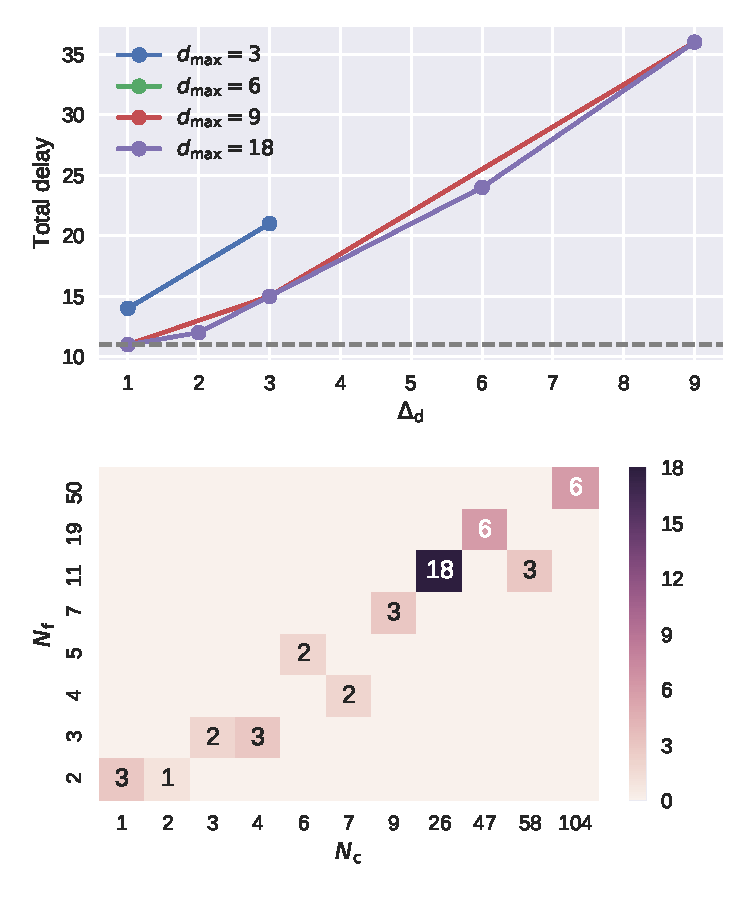
\includegraphics[width=0.45\textwidth]{./pics/delay_only_cp_results.pdf}
\caption[Effect of discretization on solution quality]{Top: Minimum total delay of a problem instance from $\mathcal{I}_{18}$ with $19$ flights and $47$ conflicts for various values of $\Delta_d$ and $d_{\max}$.
Bottom: Minimum $d_\text{max}$ necessary to obtain same optimum as that without bounding the delay for various instances in $\mathcal I_{18}$.}
\label{fig:delay_only_cp_results}
\end{figure}

Figure~\ref{fig:delay_only_cp_results} shows the minimum total delay of a problem instance with $19$ flights and $47$ potential conflicts for various values of $\Delta_d$ and $d_{\max}$.
With the exception of the small maximum delay $d_\text{max} = 3$, the total delay of the solutions is nearly independent of the maximum delay.
The total delay is non-decreasing with respect to the coarseness $\Delta_d$ of the discretization for a fixed maximum delay $d_{\max}$, and non-increasing with respect to $d_{\max}$ for a fixed $\Delta_d$.
Since the original data is discretized in time in units of $1$ minute, $\Delta_d=1$ yield the same result as a continuous variable with the same upper bound.
Above some threshold value $d^0_\text{max}$, further increasing the maximum delay does not decrease the minimum total delay.
With one exception, we found that for all the investigated problem instances $d^0_\text{max}\leq6$ minutes (see Figure~\ref{fig:delay_only_cp_results}).
Therefore we conclude, that a moderate maximum delay is sufficient even for larger problem instances.
On the other hand, the delay discretization should be as fine as possible to obtain a high quality solutions.


%%%%%%%%%%%%%%%%%%%%%%%%%%%%%%%%%%%%%%%%%%%%%%%%%%%%%%%%%%%%%%%%%%%%%%%%%%%%%%%%
% I_60
%%%%%%%%%%%%%%%%%%%%%%%%%%%%%%%%%%%%%%%%%%%%%%%%%%%%%%%%%%%%%%%%%%%%%%%%%%%%%%%%

Figure~(\ref{fig:icm1}) shows the dependence of the total delay time optimized by ICM on the delay discretization $\Delta_d$ for various problem instances extracted from the connected components of the conflict graph.
Results are for maximum delay of 60 minutes. 
As expected, the total delay decreases by decreasing $\Delta_d$.
This is consistent with the idea that smaller $\Delta_d$ allows a finer optimization of the delays of the flights.


\begin{figure}[htpb]
  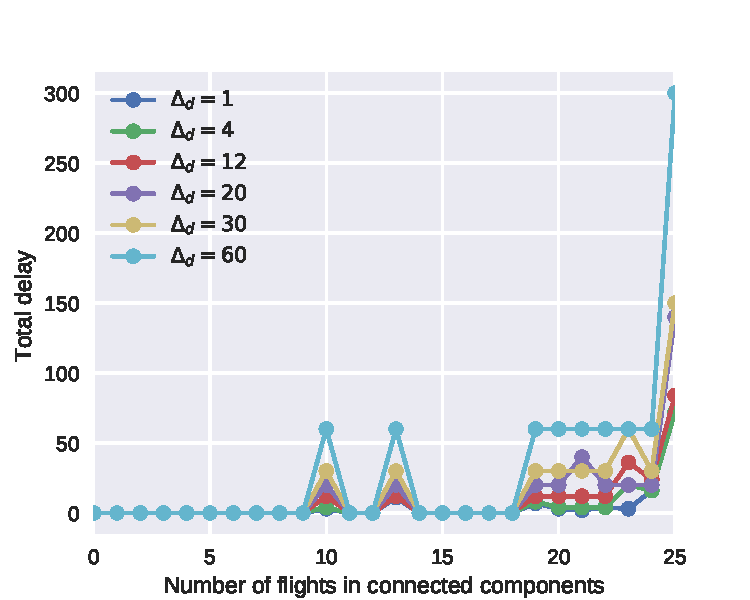
\includegraphics[width=\columnwidth]{pics/qubo_icm/qubo_icm_3.pdf}
    \caption{Total delay in dependence of the discretization parameter $\Delta_d$ for 9 different problem instances from $\mathcal{I}_{60}$ with up to in $12$ flights and $25$ conflicts.}
\label{fig:icm1}
\end{figure}

In Figure~(\ref{fig:icm2}) we show the optimal delay time found by ICM as a
function of the number of the flights in the connected components. Results are
for a maximum delay of 60 minutes. Unfortunately, ICM was unable to optimize
connected components with more than $12$ flights. This can be explained by
recalling that ICM works the best for almost-planar problem while the
its performance quickly decreases for fully-connected problems. Indeed, as shown
in Section~\ref{sec:instances}, the underlying graph of connected components
look more like a fully-connected graph rather than a tree graph by increasing
the number of flights inside the connected component.

\begin{figure}[h]
  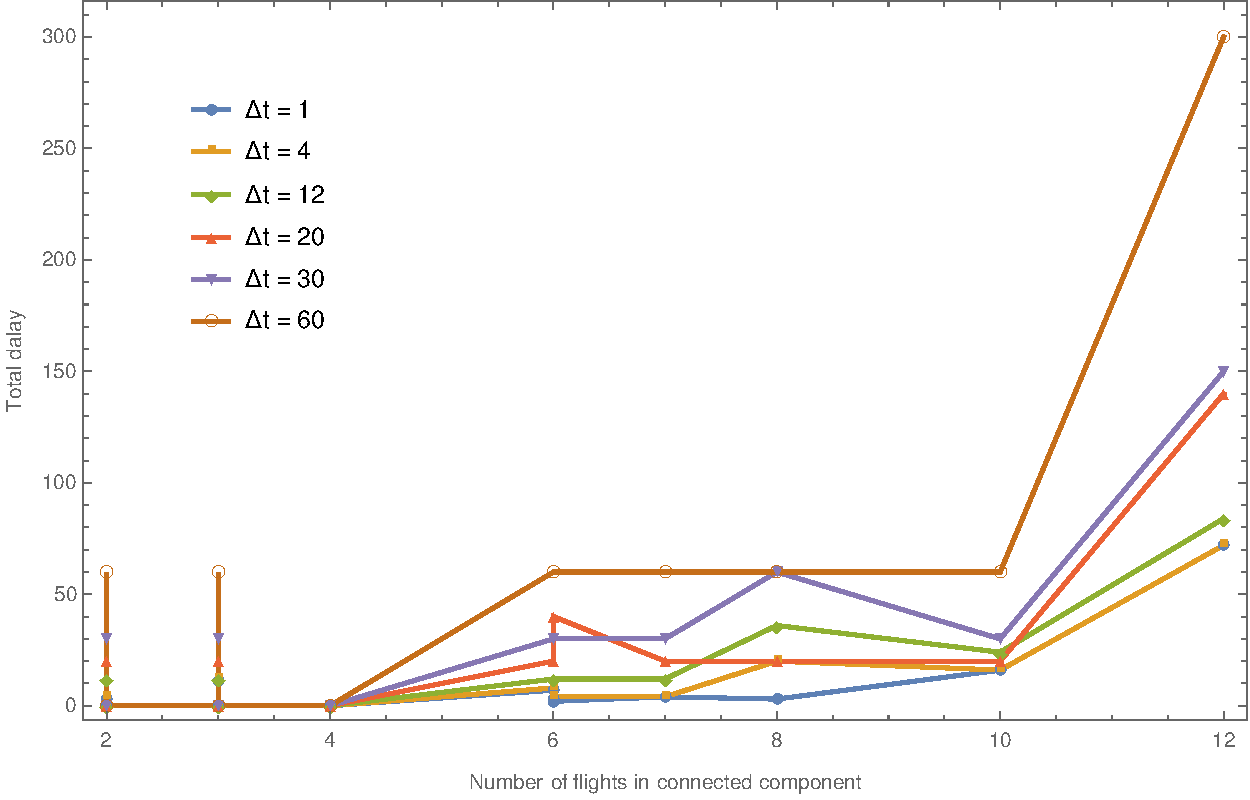
\includegraphics[width=\columnwidth]{pics/qubo_icm/qubo_icm_2.pdf}
  \caption{\label{fig:icm2}. Optimal total delay found by using the Isoenergetic
  Cluster Method (ICM) at fixed time step $\Delta_d$ as a function of numbers of
  flight within each connected component. ICM was unable to find solutions for connected
  component with more than $12$ flights.}
\end{figure}
